\documentclass{article}
\usepackage{iclr2027_conference}

\usepackage{times}
\usepackage{latexsym}
\usepackage[T1]{fontenc}
\usepackage[utf8]{inputenc}
\usepackage{microtype}
\usepackage{inconsolata}
\usepackage{graphicx}
\usepackage{booktabs}
\usepackage{amsmath}
\usepackage{hyperref}
\usepackage{url}
\hypersetup{hidelinks,pdftitle={Predicting Linear Relational Decodability Without the Relation},
  pdfauthor={},pdfsubject={},pdfkeywords={}}

\title{Predicting Linear Relational Decodability\\Without the Relation}

\author{Anonymous authors}

\newcounter{notecounter}
\newcommand{\enotesoff}{\long\gdef\enote##1##2{}}
\newcommand{\enoteson}{\long\gdef\enote##1##2{{
\stepcounter{notecounter}
{\large\bf
\hspace{0cm}\arabic{notecounter} $<<<$ ##1: ##2
$>>>$\hspace{1cm}}}}}

%\enoteson
\enotesoff

% Generated by code/scripts/build_full_evaluation_paper.py.
\newcommand{\headlinenumber}{0.735}
\newcommand{\headlinep}{8.24\times10^{-6}}
\newcommand{\capitalfaith}{87.5\%}
\newcommand{\fatherfaith}{7.5\%}



\begin{document}
\maketitle


\begin{abstract}
Linear relational embeddings (LREs) approximate a language
model's subject-to-object mapping with an affine
function. Their faithfulness varies enormously across
relations, including weak performance on \textsc{person\_father}
and stronger performance on \textsc{country\_capital\_city}. We investigate
the factors that contribute to this variation and
demonstrate that it can be significantly predicted from a
readout that is not aware of the underlying relationship. To
do so, we propose a novel form of the Jacobian lens, the
\emph{contrastive entity lens}. Whereas the Jacobian lens is estimated
across all tokens and concepts, the entity lens
$\mbox{EL}_t$
is trained
to predict what the model will output for an entity of
type $t$; e.g., we train ELs for countries and for persons.
After estimating an entity lens, we measure how
highly it ranks the model's answer for a relation -- without
using any relation-specific information in estimation and
prediction.  Across 28 relations of the LRE dataset on
Olmo-3-7B this relation-agnostic score correlates with LRE
faithfulness at $\rho = \headlinenumber$ ($p=\headlinep$),
using all 9,747 original rows, including demonstrations and references.
We report the same full-evaluation comparison for six additional models.  This association supports a role for information already carried by
the subject representation, while leaving the causal mechanism open.  At the fact level, generic first tokens and changes in the model's
answer across demonstration contexts complicate interpretation. We
report these limitations, the model-specific tokenization and prompt
corrections, and readout baselines under the same full evaluation.
\end{abstract}



\section{Introduction}

\citet{hernandez2024linearity} showed that a language model's mapping from
a subject to the object of a relation is often well approximated by an
affine function of the subject's hidden state -- a \emph{linear relational
embedding} (LRE). They also showed that this works far better for some
relations than others. On Olmo-3-7B, we reproduce the same spread: an LRE
fitted on \textsc{country\_capital\_city} agrees with the model's own
prediction \capitalfaith{} of the time while one fitted on \textsc{person\_father}
agrees \fatherfaith{} of the time in our full evaluation.

Why? The natural reading is that some relations are ``more linear'' than
others -- that linearity is a property of the relation. We report evidence
that it is better understood as a property of the \emph{subject's
representation}. Concretely, we show that one can predict how faithful an
LRE will be \emph{before fitting it}, and without using the relation at
all.

Building on recent work by \citet{gurnee2026workspace},
we introduce the \emph{contrastive entity lens} $\mbox{EL}_t$, which
is trained on subjects of type $t$ placed in the neutral prompt
\texttt{"\{\} is known for"} and
evaluates the Jacobian at entities of type $t$.
The construction changes what the readout is
about: it is not about what a model might say in general
about any concept, but about factual
knowledge and, more specifically, about factual knowledge
about an entity of a particular type.
The question it
answers -- \emph{what factual knowledge is this model ready to produce about this entity}
 -- is specific to the entity type, but not specific to any relation.

We estimate  the entity lens under the single
neutral prompt
\texttt{"\{\} is known for"} 
(shared by every relation), at one layer fixed across relations,
and ask how highly it ranks the model's own answer. The lens sees no
relation template, no objects and no (subject,~object) pairs, yet its
score correlates with LRE faithfulness across 28 relations at
$\rho = \headlinenumber $.

We make four contributions. (i)~We introduce the entity
lens, a supervision-free readout of what a model is disposed to say about
an individual entity of a specific entity type. (ii)~We turn it into a relation-agnostic diagnostic
of linear decodability and show that it predicts LRE faithfulness.
(iii)~We evaluate seven models on complete relation datasets, compare readout baselines under the same protocol, and examine controls for object cardinality and answer-token frequency.
(iv)~Moving
the unit of
analysis from the relation to the individual fact,
we provide an analysis of several
problems in existing datasets -- most prominently
semantically
weak first tokens
and reference competition --
that hinder further
progress on understanding LREs in language models. 


\section{Background}
\label{sec:background}

An LRE for relation $r$ approximates the model's computation as
\begin{equation}
o \;\approx\; \beta\, W s + b_\beta ,
\end{equation}
where $s$ is the hidden state at the subject's final token and $o$ the
output state. Write $f$ for the model's own map between the two: $f$
sends the subject's hidden state at an intermediate layer $\ell$ to the
final-layer state at the last position. We average local
first-order approximations of $f$ over a small set $\{s_i\}$ of reference
subjects and scale their subject-dependent terms by $\beta$:
\begin{equation}
W = \operatorname{mean}_i J_i , \qquad
b_\beta = \operatorname{mean}_i\!\left[\, f(s_i) - \beta J_i s_i \,\right] ,
\label{eq:wb}
\end{equation}
where $J_i$ is the Jacobian of $f$ at $s_i$. At $\beta=1$, this is the
averaged first-order Taylor approximation
\citep{hernandez2024linearity}.

This prediction decomposes into a subject-dependent term
and a constant: expanding $b_\beta$ gives
\begin{equation}
\beta W s + b_\beta \;=\;
\operatorname{mean}_i\!\left[\,f(s_i) + \beta J_i (s -
  s_i)\,\right],
\label{eq:beta}
\end{equation}
in which only the second term depends on which subject is being decoded.
Left unscaled, the shared anchor $\operatorname{mean}_i f(s_i)$ dominates
and the operator returns much the same object for every subject.
Setting $\beta > 1$ amplifies the subject-specific contribution relative
to that anchor, and so does change which object is ranked first.
\citet{hernandez2024linearity} fit $\beta$ per relation alongside the
layer; we follow their protocol and select it from
$\{0.5, 1, 1.5, 2, 3, 5\}$.




\emph{Faithfulness} is the rate at which
decoding $\beta W s + b_\beta$ over the full vocabulary reproduces the
\emph{model's own} top-1 prediction (not the gold object). It is therefore
a measure of how well an affine map captures what the model
does. Faithfulness defined this way is
the quantity we predict.

\section{Related work}

\paragraph{Linear relational embeddings.} Treating relations as linear maps
between concept representations goes back to
\citet{DBLP:conf/icml/PaccanaroH00};
\citet{hernandez2024linearity} carried the idea over
to transformer language models \citep{vaswani2017attention}, and
subsequent work has asked why the resulting LREs are faithful for some
relations and not others.
\citet{merullo2025linear} trace part of this
variation to pretraining data: LREs are more faithful when subjects and
objects frequently co-occur in the corpus (we compare against such
frequency measures in Appendix~\ref{sec:corpus-freq-baselines}). A further question is whether such
structure reflects what a model has learned or only the particular
parametrization that realizes it, since many parametrizations induce the
same next-token distribution. Existing results point to the former,
since under suitable conditions, relational linearity holds either in
all distribution-equivalent models or in none, and it has been shown
empirically, through a probe based on the Kullback--Leibler divergence,
to vary across models, layers and phrasings of the relation
\citep{marconato2024all, valer2026relational}.
These works evaluate and explain linearity at the level of the relation.
We ask instead how much of it can be predicted from how the model
represents the subject, using a readout estimated without the relation
or any of its objects.

\paragraph{Subject representations in factual recall.} Mechanistic studies
converge on the view that much factual knowledge is attached to the
subject before the relation is processed. Feed-forward layers operate as
key--value memories whose keys respond to patterns in the input and
whose values induce distributions over the output vocabulary, and in
middle layers at the last subject token they are where causal tracing
localizes factual associations and where targeted edits change
individual facts
\citep{geva2021transformer, meng2022locating}.
Building on these findings, factual recall has been decomposed into
stages: MLP layers enrich the subject representation with many of its
attributes, a lookup that depends largely on the subject's name rather
than on the preceding context; the relation is propagated to the final
position; and attention heads extract the requested attribute
\citep{geva-etal-2023-dissecting, nanda2024fact}.
\citet{10.1162/TACL.a.746} show that knowledge
acquisition tracks how often subject and answer co-occur, though
frequency alone does not fully explain learning, which is why we treat
the corpus-frequency baselines in Appendix~\ref{sec:corpus-freq-baselines} as a comparison rather
than an explanation. Our approach can be read as a probe of this
enrichment, since it reports what the model is prepared to say about a
subject before any relation is given. This allows us to connect two
lines of work: We hypothesize that the enrichment the lens diagnoses
contributes to the relational linearity found by
\citet{hernandez2024linearity}. The lens predicts LRE
faithfulness across relations in all seven models we test, and the
association persists when controlling for object cardinality and
answer-token frequency (§\ref{sec:results}).

\paragraph{How facts are stored.} Theoretical work offers two accounts of
how transformers store facts.
\citet{nichani2025understanding} model attention and MLP
weights as associative memories and prove that a one-layer transformer
can store a number of facts that scales linearly with its parameter
count, with storage traded off between self-attention and MLP
parameters. \citet{DBLP:journals/corr/abs-2605-12426} study a
geometric form of storage: in a controlled one-layer setting, subject
embeddings encode linear superpositions of their associated attributes,
and a small MLP selects among them conditioned on the relation. In
pretrained models the two need not compete: lookup-like computation can
enrich the subject representation over the early and middle layers, and
the geometric picture then describes the enriched state from which a
relation selects. Our hypothesis concerns this enriched state: a
relation should be linearly decodable to the extent that its attribute
is prominently encoded in the subject representation after enrichment.

\paragraph{Lenses.} Lenses read out intermediate hidden states in terms of
the output vocabulary and differ mainly in the map they apply: the
model's own unembedding
\citep{nostalgebraist2020interpreting}, an affine translator
learned per layer \citep{belrose2023eliciting}, or
the model's input--output Jacobian averaged over a large corpus and
applied to raw activations, with the aim of identifying representations
the model is poised to verbalize
\citep{gurnee2026workspace}.
Our entity lens instead evaluates the Jacobian at reference entities of
the subject's type under a single neutral factual prompt, so that the
readout concerns what the model is prepared to say about entities of
that type rather than about any concept. Its contrastive variant further
applies the Jacobian to differences between entity representations,
subtracting what the references share.



%\citet{DBLP:conf/icml/PaccanaroH00} introduce linear
%relational embeddings (LREs)
%and \citet{hernandez2024linearity} show that LREs are part
%of the mechanism by which transformer models answer factual questions.
%
%
%\citet{merullo2025linear} show that the frequency
%of subject-object cooccurrence
%in the
%pretraining corpus is an important determinant of
%linearity. In our work, we put forward the hypothesis that
%relational linearity is primarily a property of how the model
%represents the subject, independent of the relation (or object). We also
%identify object cardinality as an additional important
%variable for linearity. Finally, we analyze limitations of
%LRE for understanding linearity and make suggestions for how
%future factual recall datasets should be constructed for
%relational linearity research.
%
%\citet{geva-etal-2023-dissecting} proposes subject
%enrichment as a key mechanism for factual recall. We can
%interpret our contrastive Jacobian lens as a probe of
%subject enrichment.
%Crucially, we connect in this paper two different lines of
%research on the representation of relations in transformer
%models: we hypothesize that the type of subject enrichment that the Jacobian
%lens diagnoses gives rise to the linearity of relations
%found by \citet{hernandez2024linearity}.
%
%DISCUSS \cite{10.1162/TACL.a.746}
%
%DISCUSS \cite{DBLP:journals/corr/abs-2605-12426}



\section{The entity lens}
\label{sec:lens}
\enote{sg}{I think the whole CEL stuff is something we could move to the appendix, so the reader can focus on NEL which now seems to be the main thing.}


\citet{gurnee2026workspace}'s Jacobian lens is broadly
similar to LRE.  But
instead of a relation-specific prompt and a focused target
position (the object),
it computes the average 
$W = \operatorname{mean}_i J_i$ over many diverse prompts and many
output positions. The Jacobian lens also does not use the
``anchor'', the zero-order term of the Taylor expansion; so it
is simply $W = \operatorname{mean}_i J_i$.

We derive our \emph{contrastive entity lens} from
Eq.~\ref{eq:beta}, restated as:
\begin{equation}
  f(s) \approx
\beta W s + b_\beta \;=\;
\operatorname{mean}_i\!\left[\,f(s_i)\right]
+ \beta\operatorname{mean}_i\!\left[\, J_i (s - s_i)\,\right]
\end{equation}
Following \citet{gurnee2026workspace}, we also drop the anchor
term $\operatorname{mean}_i\!\left[\,f(s_i)\right]$; see discussion in 
\S\ref{sec:swap}.
This also means that we do not need $\beta$ since the
scaling does not change the output distribution over
tokens. The final form of the contrastive entity lens is then:
\begin{equation}
\mbox{CEL}(e) = \operatorname{mean}_i\!\left[\, J_i (s_e - s_i)\,\right]
\label{eq:cel}
\end{equation}
CEL takes into account the difference between $s_e$ and
the reference point $s_i$, as it should if we want
to approximate $f(s_e)$ using the first derivative. 
Our original motivation was that we are not interested in what the model associates
with an entity like ``Russia'' in general (e.g.,
``Europe''). Instead we are interested in what the model
associates with ``Russia'', but not with other reference
entities like ``Spain'' and ``Italy''. Examples of such
contrastive associations for ``Russia'' are ``vodka'' and ``Kremlin''.
Our hypothesis was that such top-ranked contrastive associations
give rise to linearity.

In initial experiments, we found that the contrastive entity
lens is quite sensitive to the reference set. For example,
if $s_e$ is a French person and a Spanish person is the
reference entity $s_i$, then the vector difference in 
Eq.~\ref{eq:cel} will enhance ``French''. But if $s_i$ is
another French person, then ``French'' will be demoted.
This is bad for answering questions about $s_e$'s
nationality and native language. We therefore also consider
the following noncontrastive entity lens, which drops the
reference set differences:
\begin{equation}
\mbox{NEL}(e) = \operatorname{mean}_i\!\left[\, J_i s_e \,\right]
\label{eq:nel}
\end{equation}
In what follows,
EL refers to both NEL and CEL.

% and
%``entity lens'' refers to NEL unless
%further specified.

To instantiate EL for factual
relations, we need (i) a prompt that evokes factual associations
and (ii) a reference set of entities for computing the Jacobians $J_i$
(both NEL and CEL) and for serving as the $s_i$ in the
vector differences $s_e - s_i$ (for CEL).

As the prompt we adopt \texttt{"\{\} is known for"}. This is a neutral prompt, i.e.,
it is not customized for any specific factual relation. We
use it for all our  experiments unless otherwise stated.

As the reference set, we use entities of the same type as
the subject, e.g., other countries if the subject is a
country, other landmarks if the subject is a landmark
etc.
NEL applied to an input $s$ outputs anything the model is likely
to say in a context in which an entity of the same type as $s$ occurs, including features
it shares with other same-type entities.
CEL outputs only what differentiates
$s$ from other same-type entities.

\paragraph{Computation.} We do not compute $J_i$ explicitly, but obtain each
Jacobian--vector product $J_i u$ by the double-backward
construction \citep{pearlmutter1994fast}, at the cost of a constant
number of forward and backward passes (Appendix~\ref{sec:jvp}).


%; this is what makes
%Eq.~\ref{eq:cel} affordable at $d_{\text{model}}=4096$

\enote{hs}{is this clearly stated in this section? or do we
  need to repeat it here?
\paragraph{What makes $A_r$ relation-agnostic.} Eq.~\ref{eq:cel} is not specific to $r$: the prompt is neutral and shared,
the layer is fixed at 17 for all relations
(Appendix~\ref{sec:layer17}) and
no (subject,~object) pair of the
relation is used in estimation.
}





\section{Experimental setup}
\label{sec:setup}

\paragraph{Models and relations.} We evaluate OLMo 3 7B, GPT-J 6B,
Pythia 6.9B, Mistral 7B, Gemma 2 9B, Qwen3 8B Base and Qwen3.8 27B,
using pinned checkpoints in \texttt{float32} with eager attention.
OLMo is the main worked example. We retain the original 28 named-entity
relations from the LRE dataset \citep{hernandez2024linearity}, comprising
9,747 rows, including duplicates. We do not expand to the other 19
relations or filter rows by correctness or first-token uniqueness.
The model-specific year exception is documented in
Appendix~\ref{sec:full-protocol}.

\paragraph{Full evaluation.} Each method retains its original reproducible
selection of eight in-context demonstrations and eight reference rows.
Every original row is evaluated, including demonstrations and references.
The two methods use different seeded demonstration/reference selections;
their evaluation multisets are identical, but their relation-context
answer tokens can differ. The in-context prompt contains eight
(subject, object) examples and a query subject without its answer.
The lens uses this context only to obtain its target token; its hidden
states and Jacobians always come from the neutral prompt.

For LRE, a six-layer by six-scaling grid selects the most faithful
operator on the full evaluation. The scaling candidates are
$\{0.5,1,1.5,2,3,5\}$; the model-specific layer grids and fixed lens layers
are listed in Appendix~\ref{sec:layer17}. The lens omits self-reference
comparisons for a query subject, but retains the query row in scoring.
These are explicitly \emph{in-sample} results: both reference/example
reuse and LRE parameter selection involve evaluated rows. They do not
estimate generalization to an independent held-out set.

\paragraph{Scoring corrections.} Gender answers use the established
same-gender alternative wording sets for lens ranks. LRE faithfulness
remains exact agreement with the model's top-1 token. Continent references
use the original seeded selection, without rebalancing. For GPT-J,
Pythia and the two Qwen models, the neutral prompt starts with a newline:
\texttt{\textbackslash n\{\} is known for}. This avoids the large
subject-state norms observed at the first token. The model names are
marked in Table~\ref{tab:full-models}; Appendix~\ref{sec:full-protocol}
records all corrections and their scope.

\section{Results}
\label{sec:results}

\begin{figure}[t]
\centering
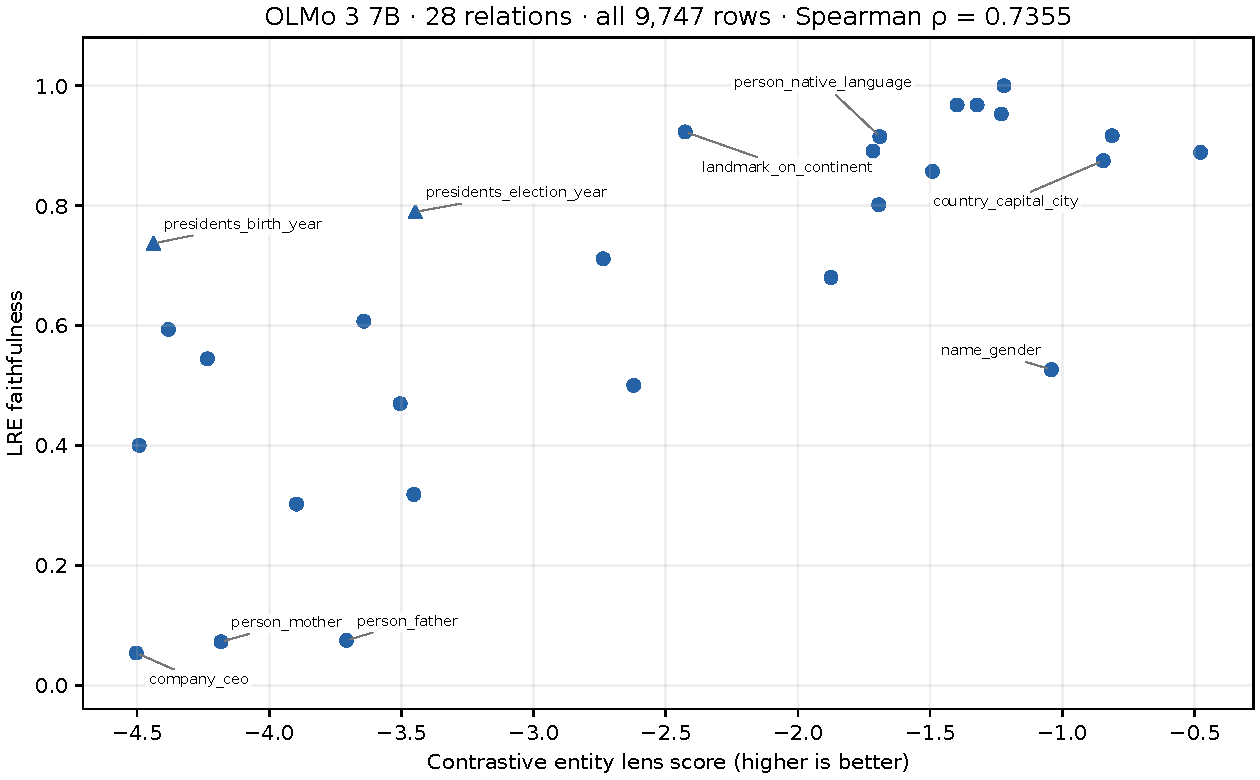
\includegraphics[width=\linewidth]{fig_full_evaluation.pdf}
\caption{OLMo contrastive entity lens score against full-evaluation LRE
faithfulness for all 28 relations and 9,747 rows. Every original row is
included, with gender alternatives enabled and original continent
references. Triangles mark the two year relations, retained after
checking their token boundaries. Labels identify the residual extremes
and relations discussed in the text.}
\label{fig:main}
\end{figure}

Figure~\ref{fig:main} gives Spearman $\rho=\headlinenumber$
($p=\headlinep$) for OLMo. Table~\ref{tab:full-models} reports the same
contrastive/differential readout for every model. The correlation is
positive across the models but varies in magnitude. This is evidence
that the relation-agnostic readout carries information about LRE
faithfulness; it does not show that all models use an identical mechanism.

% Generated by code/scripts/build_full_evaluation_paper.py.
\begin{table}[t]
\centering\small
\caption{Full-evaluation contrastive/differential Jacobian lens correlations with LRE faithfulness. LRE layer and scaling are selected on the full evaluation grid.}
\label{tab:full-models}
\begin{tabular}{@{}lrrrr@{}}
\toprule
Model & Relations & Scored rows & Spearman $\rho$ & $p$ \\
\midrule
OLMo 3 7B & 28 & 9,747 & $0.7355$ & $8.24\times10^{-6}$ \\
GPT-J 6B$^{\dagger}$ & 28 & 9,747 & $0.4346$ & $0.021$ \\
Pythia 6.9B$^{\dagger}$ & 28 & 9,747 & $0.5027$ & $0.006$ \\
Mistral 7B & 26 & 9,709 & $0.6561$ & $2.74\times10^{-4}$ \\
Gemma 2 9B & 26 & 9,709 & $0.6889$ & $9.96\times10^{-5}$ \\
Qwen3 8B Base$^{\dagger}$ & 26 & 9,709 & $0.6647$ & $2.12\times10^{-4}$ \\
Qwen3.8 27B$^{\dagger}$ & 26 & 9,709 & $0.5539$ & $0.003$ \\
\bottomrule
\end{tabular}
\par\smallskip\begin{minipage}{\linewidth}\footnotesize $^{\dagger}$Leading newline in the neutral lens prompt to address high first-position activation norms. All eligible rows, including demonstration/reference rows, are evaluated. Models with 26 scored relations exclude the two year relations whose first answer token is the standalone digit 1; all 28 relations were measured. Gender alternatives are enabled; continent references use the original seeded selection.\end{minipage}
\end{table}


\paragraph{Controls.}
% Generated by code/scripts/build_full_evaluation_paper.py.
Across all 28 OLMo relations, cardinality has Spearman $\rho=0.355$ with faithfulness ($p=0.064$) and $\rho=0.086$ with the lens score. The partial Spearman correlation controlling for cardinality is $0.757$ ($p=4.90\times10^{-6}$).

Answer-token prior has Spearman $\rho=-0.111$ with faithfulness and $\rho=0.098$ with the lens score. Controlling for this prior gives $\rho=0.755$; controlling for both prior and cardinality gives $\rho=0.784$ ($p=2.14\times10^{-6}$). The prior is the mean log probability of each evaluation target under ten neutral contexts, averaged over every original row.

For partial correlations, we rank-transform both scores and each
covariate, regress each score on the covariates with an intercept, and
correlate the residuals. All controls use the complete 28-relation OLMo
evaluation; no small-test-size cohort is selected.

\paragraph{Readout and frequency baselines.} Appendix~\ref{sec:shared-baselines}
compares the contrastive lens with the noncontrastive Jacobian lens,
logit lens, differential logit lens and a Wikipedia attribute measure.
Each comparison uses the same model-specific full evaluation and
corrections. The contrastive lens does not uniformly outperform these
baselines: the noncontrastive lens is stronger for several models, and
ordinary logit lens has the largest point correlation among the
vocabulary-rank readouts for GPT-J and Qwen3 8B Base. These comparisons
do not establish statistically significant differences between readouts.
OLMo corpus-frequency features are reaggregated over all
original rows before correlation with the current faithfulness values.

\section{Analysis of the entity lens}
\subsection{Neutral prompts and reference composition}
\label{sec:salience}
The neutral prompt asks what an entity is known for. Its readout may
therefore emphasize identity, profession or cultural associations while
ranking gender, family members or university names poorly. We interpret
this as a possible limitation of the probe, not proof that those facts
are absent from the representation. The present results do not establish
that salience is the causal mechanism behind LRE faithfulness.

\subsection{Reference sets}
\label{sec:refsets}
The contrastive readout averages $J_i(s_e-s_i)$ over reference entities
of the same subject type. If a queried subject and its references share
an answer-related direction, subtraction can suppress that direction.
The noncontrastive readout $\operatorname{mean}_i J_i s_e$ does not perform
this subtraction; we compare it under the same full-evaluation protocol
in Appendix~\ref{sec:shared-baselines}.

The current measurements retain the original seeded reference rows,
including their answer-category imbalance. In particular, the
landmark-continent reference sets are not balanced across continents.
This makes the choice reproducible, but it does not make the references
neutral with respect to every relation. Reference-composition robustness
is not established by the present aggregate correlations.


\section{Relation-level outliers}
\label{sec:residuals}
We fit a least-squares line to the OLMo points in Figure~\ref{fig:main}
and inspect residuals in units of faithfulness.
% Generated by code/scripts/build_full_evaluation_paper.py.
The largest positive residuals are \textsc{presidents\_birth\_year} ($+0.375$, $k=1.3$), \textsc{presidents\_election\_year} ($+0.271$, $k=1.1$), \textsc{landmark\_on\_continent} ($+0.242$, $k=189.4$). The largest negative residuals are \textsc{person\_father} ($-0.403$, $k=1.0$), \textsc{name\_gender} ($-0.374$, $k=9.5$), \textsc{person\_mother} ($-0.330$, $k=1.0$). These residuals are recomputed from the least-squares fit to the full-evaluation points; they are measured in faithfulness units.

These examples show why cardinality and lens agreement need not have the
same association with faithfulness. Repeated answer tokens can make an
operator faithful without fine-grained subject discrimination, whereas a
large answer space makes exact top-1 agreement difficult. The residuals
are descriptive; the full-data controls in Section~\ref{sec:results}
do not establish a causal explanation for either tail.

\section{Fact-level analysis}
\label{sec:subject}
% Generated by code/scripts/build_full_evaluation_paper.py.
We join all 9,747 OLMo evaluation rows by subject and object, retaining duplicate occurrences, and correlate the two answer-token ranks within each relation. Correlations are defined for 27 of 28 relations, ranging from $-0.401$ to $0.664$, with median $0.235$ among defined relations. Constant ranks make the statistic undefined for \textsc{country\_language}; their rows are retained in every other analysis. The two methods use different demonstration contexts, whose target tokens disagree on 2,115 of these rows. These within-relation associations therefore combine readout differences with context sensitivity; they do not compare an identical target under matched contexts.

Appendix~\ref{sec:full-facts} lists every relation, including undefined
correlations caused by constant ranks.

\subsection{Context and entity ambiguity}
\label{sec:competition}
A subject string can evoke more than one entity, and the neutral prompt
can emphasize associations other than the requested relation. Different
in-context examples can also change the model's answer. Both issues
complicate an interpretation of rank disagreement as evidence that a
fact is missing from a linear representation. A future matched-context
experiment should separate these effects while retaining the complete
evaluation; the current protocol preserves the original contexts.

\subsection{Semantically weak first tokens}
The first token of a multi-token answer can be shared by many distinct
objects. University names provide a concrete full-evaluation example:
the selected GPT-J LRE predicts ``University'' for every one of the 91
rows and obtains 79.1\% faithfulness; Pythia does the same and obtains
85.7\%. These scores exactly match their constant majority-token
baselines. Thus high faithfulness can reflect agreement on a generic
prefix rather than recovery of a university's identity.
This issue persists after the newline correction. We retain these rows
and report the limitation instead of filtering away inconvenient
objects or model predictions.

\subsection{Towards better fact evaluations}
Answer scoring should distinguish complete objects rather than credit a
shared, semantically weak first token. Complete-answer scoring is a
separate metric and is not substituted into the present first-token
faithfulness results. Likewise, evaluations should distinguish ambiguity
in the intended subject from failure of the relational readout, and
should report when their demonstration contexts induce different targets.

\section{Interpreting the operator's two terms}
\label{sec:swap}
The affine operator in Eq.~\ref{eq:wb} separates a subject-dependent term
$\beta W s$ from an anchor $b_\beta$ fixed by the references. This algebra
motivates comparisons with neutral-prompt Jacobian readouts, but it does
not show that a neutral readout can substitute for the subject term of a
relation-context LRE. We therefore interpret the full-evaluation
correlations as predictive associations. Establishing interchangeable
terms would require an intervention study with explicit complete-data
coverage and scoring, beyond the comparisons reported here.


\section{Limitations}
\label{sec:limitations}
The benchmark covers seven models and 28 original relations, with two
model-specific year exclusions in four models. It remains a small
relation-level sample, and related datasets can share subjects and
objects. Correlations and unadjusted $p$-values are descriptive evidence
rather than an identification of causal mechanisms.

The evaluation includes demonstration and reference rows and selects
LRE layer/scaling on the scored data. This improves coverage of small
relations but creates in-sample dependence; the reported correlations
must not be read as independent held-out performance. Gender has only
19 rows, including a duplicate, even under complete evaluation.

The neutral prompt, reference composition and fixed lens layer all
influence the readout. Newline corrections were motivated by activation
norm diagnostics and evaluated on these same relations. We do not claim
an independent validation of their effect or robustness across arbitrary
neutral prompts. First-token scoring can still reward generic prefixes,
and different demonstration contexts can change the two methods' target
tokens. Complete-answer and matched-context evaluation remain open work.

\section{Conclusion}
A contrastive Jacobian readout computed under a neutral prompt predicts
variation in LRE faithfulness across complete relation evaluations.
The association holds across seven models, with the largest first-token
norm artifacts reduced by a leading newline where needed. Its magnitude
and its outliers depend on the model and scoring protocol. Full-row
coverage, explicit tokenization corrections and aligned baseline
protocols are necessary for interpreting this evidence.

\label{sec:main-end}
\clearpage

\section*{AI use statement}
We used generative AI tools for brainstorming, assisting with software code, and initial drafting and rewriting of parts of the manuscript. All AI-assisted code and text were reviewed and verified by the authors, and generated code was tested for correctness. The authors take responsibility for the final content of this work, including all text, claims, results, and artifacts produced with the aid of generative AI.

\section*{Reproducibility statement}
We provide sufficient details to reproduce all experiments in the main text and appendix, including the datasets, model checkpoints, prompt templates, evaluation procedures, and hyperparameters used throughout. All experiments use publicly available model checkpoints and datasets. We report the procedures used to estimate linear relational embeddings and the contrastive Jacobian lens, as well as the definitions of all faithfulness and ranking metrics. Additional implementation details, robustness analyses, and per-relation results are provided in the appendix. Code for reproducing the experiments and figures will be released upon publication.

\bibliographystyle{iclr2027_conference}
\bibliography{custom}

\clearpage
\appendix


\section{Baseline comparisons}
\label{sec:shared-baselines}
% Mention and reference the exact Tables i.e Table X and Y show 
The first two tables report Spearman correlations with LRE faithfulness across the LRE Dataset.


% Generated by code/scripts/format_shared_baseline_tables.py.
\begin{table}[!htbp]
\centering
\caption{\textbf{Readout baselines across seven models.} Spearman correlation $\rho$ with LRE faithfulness.}
\label{tab:shared-lenses-spearman}
\begingroup
\small
\renewcommand{\arraystretch}{1.18}
\setlength{\tabcolsep}{3pt}
\begin{tabular*}{\linewidth}{@{\extracolsep{\fill}}lrrrrr@{}}
\toprule
Model & \shortstack[r]{Differential\\Jacobian} & \shortstack[r]{Raw\\Jacobian} & Logit lens & \shortstack[r]{Differential\\logit lens} & \shortstack[r]{Attribute\\rate} \\
\midrule
OLMo 3 7B & $\phantom{-}0.7355$ & $\phantom{-}\mathbf{0.7650}$ & $\phantom{-}0.2056$ & $\phantom{-}0.4390$ & $-0.4016$ \\
GPT-J 6B & $\phantom{-}0.4346$ & $\phantom{-}0.4196$ & $\phantom{-}\mathbf{0.4669}$ & $\phantom{-}0.2020$ & $-0.1035$ \\
Mistral 7B & $\phantom{-}0.6561$ & $\phantom{-}\mathbf{0.6711}$ & $\phantom{-}0.6581$ & $\phantom{-}0.5186$ & $-0.2202$ \\
Gemma 2 9B & $\phantom{-}\mathbf{0.6889}$ & $\phantom{-}0.6868$ & $\phantom{-}0.4728$ & $\phantom{-}0.3436$ & $-0.5515$ \\
Qwen3 8B Base & $\phantom{-}0.6647$ & $\phantom{-}0.6232$ & $\phantom{-}\mathbf{0.7908}$ & $\phantom{-}0.5952$ & $-0.0557$ \\
Qwen3.8 27B & $\phantom{-}0.5539$ & $\phantom{-}\mathbf{0.5717}$ & $\phantom{-}0.3404$ & $\phantom{-}0.4492$ & $-0.0099$ \\
Pythia 6.9B$^{\dagger}$ & $\phantom{-}0.5027$ & $\phantom{-}\mathbf{0.5063}$ & $-0.2047$ & $\phantom{-}0.1845$ & $\phantom{-}0.0041$ \\
\bottomrule
\end{tabular*}
\endgroup
\par\vspace{5pt}
\begin{minipage}{\linewidth}\footnotesize
Bold marks the largest point estimate within each model, not a significant difference. $^{\dagger}$Pythia's attribute rate excludes 413 test rows with no predictions surviving the attribute filter; the other models have no undefined rates.
\end{minipage}
\end{table}


\paragraph{Readout definitions.}
For subject state $s_e$, reference states $s_i$, and reference Jacobians
$J_i$, the contrastive and noncontrastive entity lenses decode
$\operatorname{mean}_i J_i(s_e-s_i)$ and
$\operatorname{mean}_i J_i s_e$, respectively. Logit lens decodes $s_e$;
differential logit lens decodes $s_e-\operatorname{mean}_i s_i$. Each relation's score is the negative median $\log_{10}(\mathrm{rank}+1)$ of the model's answer token.

\paragraph{Attribute rate.}
Following \citet{geva-etal-2023-dissecting}, we measure overlap between filtered top-50
logit-lens predictions and subject attributes retrieved from Wikipedia.
The index uses the union of current test subjects; the source stopword,
length, and retrieval filters are retained. Relation scores average the
percentage overlap. Undefined rates are handled as noted in the table;
matched-row sensitivity results remain in the accompanying data.

NEL has a larger point estimate than CEL in four models. All seven paired 95\% relation-bootstrap intervals for their
difference include zero; these results do not establish a general advantage
for either readout. LRE hyperparameter selection remains in sample.

\clearpage
\subsection{OLMo corpus-frequency baselines}
\label{sec:corpus-freq-baselines}

% Generated by code/scripts/format_shared_baseline_tables.py.
\begin{table}[!htbp]
\centering
\caption{\textbf{Frequency baselines for OLMo 3 7B.} Correlations with LRE faithfulness using document counts from OLMo's three published training mixes combined.}
\label{tab:shared-corpus-spearman}
\begingroup
\small
\renewcommand{\arraystretch}{1.16}
\setlength{\tabcolsep}{6pt}
\begin{tabular*}{\linewidth}{@{\extracolsep{\fill}}lrr@{}}
\toprule
Frequency measure & Spearman $\rho$ & $p$-value \\
\midrule
\multicolumn{3}{@{}l}{\textit{Marginal frequencies}} \\
\addlinespace[2pt]
Subject frequency, $c_s$ & $\phantom{-}0.1380$ & $0.484$ \\
Object frequency, $c_o$ & $\phantom{-}0.5712$ & $0.001$ \\
\addlinespace[5pt]
\multicolumn{3}{@{}l}{\textit{Co-occurrence}} \\
\addlinespace[2pt]
Joint frequency, $c_{so}$ & $\phantom{-}0.4568$ & $0.015$ \\
Mean of $\log(1+c_{so})$ & $\phantom{-}0.4191$ & $0.026$ \\
$\log(1+\mathrm{mean}(c_{so}))$ & $\phantom{-}0.4568$ & $0.015$ \\
\addlinespace[5pt]
\multicolumn{3}{@{}l}{\textit{Conditional frequencies}} \\
\addlinespace[2pt]
Forward conditional, $P(o\mid s)$ & $\phantom{-}0.4486$ & $0.017$ \\
Reverse conditional, $P(s\mid o)$ & $-0.4149$ & $0.028$ \\
Directional difference, $P(o\mid s)-P(s\mid o)$ & $\phantom{-}0.4826$ & $0.009$ \\
Micro-averaged $P(o\mid s)$ & $\phantom{-}0.5504$ & $0.002$ \\
Micro-averaged $P(s\mid o)$ & $-0.1453$ & $0.461$ \\
\bottomrule
\end{tabular*}
\endgroup
\par\vspace{5pt}
\begin{minipage}{\linewidth}\footnotesize
Counts denote binary document presence. Means use the current test rows with both marginals observed; micro averages are ratios of summed counts. The $p$-values are two-sided and unadjusted.
\end{minipage}
\end{table}


\paragraph{Counting and aggregation.}
A document contributes at most one mention per subject/object string.
Matching uses normalized literal names with Unicode word boundaries,
without alias resolution or a proximity constraint. With subject, object,
and joint counts $c_s$, $c_o$, and $c_{so}$, the conditionals are
$P(o\mid s)=c_{so}/c_s$ and $P(s\mid o)=c_{so}/c_o$.
Macro features average row-level quantities where both marginals are
observed. Micro conditionals divide summed joint counts by summed
marginals. The log of the mean joint count has the same Spearman correlation
as the mean joint count because the transformation is monotonic.

\paragraph{Interpretation and reproducibility.}
These are exploratory associations. Relations can share subjects and
objects, and the reported $p$-values are unadjusted. Conditional direction
also reflects marginal frequency: when $c_{so}>0$, $P(o\mid s)/P(s\mid o)=c_o/c_s$.


\clearpage
\subsection{Neutral-prompt variations}
\label{sec:prompt-variations}

Table~\ref{tab:shared-prompt-variations} reports prompt variations for the
Qwen3 8B Base contrastive entity lens. We tested these variations because
initial correlations were low with the neutral prompt used for OLMo,
\texttt{\{s\} is known for}. All prompts use the same checkpoint,
layer 19, demonstrations, reference sets, 9,747 evaluation rows, gender scoring,
relation-prompt answer tokens, and LRE outcomes as
Table~\ref{tab:shared-lenses-spearman}. Correlations use the same 26 relations
after the model's two year-relation exclusions. Only the displayed neutral
prompt varies; \texttt{\textbackslash n} denotes one leading newline.

After observing unusually large subject-state norms at position zero, we
added a leading newline (\texttt{\textbackslash n}) to the original prompt.
This moves every subject past position zero while preserving Qwen's original
token sequence. The table marks this control with $\dagger$.

% Generated by code/scripts/format_prompt_variation_table.py.
\begin{table}[!htbp]
\centering
\caption{\textbf{Neutral-prompt variations.} Spearman $\rho$ between differential-Jacobian scores and retained LRE faithfulness. Panel A compares exact templates for Qwen3 8B Base; panel B isolates the newline-prefix comparison across all seven models on the shared split.}
\label{tab:shared-prompt-variations}
\begingroup
\small
\renewcommand{\arraystretch}{1.16}
\setlength{\tabcolsep}{5pt}
\begin{tabular*}{\linewidth}{@{\extracolsep{\fill}}lrr@{}}
\toprule
\multicolumn{3}{@{}l}{\textbf{A. Qwen3 8B Base: prompt wording and prefix}} \\
\addlinespace[3pt]
Neutral prompt & Shared ($n=25$) & Legacy ($n=28$) \\
\midrule
\texttt{\{s\} is known for} & $\phantom{-}0.268$ & $\phantom{-}0.060$ \\
\texttt{\{s\}} & $-0.057$ & $\phantom{-}0.058$ \\
\texttt{\{s\} is} & $\phantom{-}0.166$ & $-0.118$ \\
\texttt{\{s\} can be described as} & $\phantom{-}0.372$ & $\phantom{-}0.179$ \\
\texttt{Information about \{s\}:} & $\phantom{-}0.733$ & $\phantom{-}0.295$ \\
\texttt{Facts about \{s\}:} & $\phantom{-}0.788$ & $\phantom{-}0.298$ \\
\texttt{Entity: \{s\} is known for} & $\phantom{-}0.728$ & $\phantom{-}0.202$ \\
\addlinespace[4pt]
\texttt{\textbackslash n\{s\} is known for} & $\phantom{-}0.729$ & $\phantom{-}0.216$ \\
\bottomrule
\end{tabular*}
\par\vspace{10pt}
\begin{tabular*}{\linewidth}{@{\extracolsep{\fill}}lrrr@{}}
\toprule
\multicolumn{4}{@{}l}{\textbf{B. All models: newline prefix, shared split ($n=25$)}} \\
\addlinespace[3pt]
Model & Original & Newline & $\Delta\rho$ \\
\midrule
OLMo 3 7B & $\phantom{-}0.624$ & $\phantom{-}0.683$ & $+0.058$ \\
GPT-J 6B & $\phantom{-}0.155$ & $\phantom{-}0.573$ & $+0.418$ \\
Mistral 7B & $\phantom{-}0.625$ & $\phantom{-}0.606$ & $-0.018$ \\
Gemma 2 9B & $\phantom{-}0.487$ & $\phantom{-}0.554$ & $+0.066$ \\
Qwen3 8B Base & $\phantom{-}0.268$ & $\phantom{-}0.729$ & $+0.461$ \\
Qwen3.8 27B & $\phantom{-}0.596$ & $\phantom{-}0.600$ & $+0.003$ \\
Pythia 6.9B & $-0.045$ & $\phantom{-}0.479$ & $+0.524$ \\
\bottomrule
\end{tabular*}
\endgroup
\par\vspace{5pt}
\begin{minipage}{\linewidth}\footnotesize
$s$ denotes the subject; \texttt{\textbackslash n} denotes one leading newline. Panel B compares \texttt{\{s\} is known for} with \texttt{\textbackslash n\{s\} is known for}. The newline is a position control measured after the seven-template Qwen comparison; no additional newline is implied for the other templates.
\end{minipage}
\end{table}


\clearpage



\section{Jacobian--vector products}
\label{sec:jvp}

Neither the operator nor the lens ever needs $J_i$ itself, only products
$J_i u$: for the lens this is explicit in Eq.~\ref{eq:cel}, and for the
LRE it is what the expansion in Eq.~\ref{eq:beta} buys, since it turns
$W = \operatorname{mean}_i J_i$ into a sum of such products. We obtain
each one by the standard
double-backward construction \citep{pearlmutter1994fast}: differentiate
$\langle u', f(h)\rangle$ with respect to $h$ with $u'$ held as a free
variable, then differentiate the result with respect to $u'$ in the
direction $u$. Each product therefore costs a constant number of forward
and backward passes rather than the $d_{\text{model}}$ passes a
materialized Jacobian would need. The construction requires
\texttt{float32} and eager attention, as the fused attention kernels are
not twice differentiable.

\section{Layer selection}
\label{sec:layer17}
The lens uses one fixed intermediate layer per model, with no
per-relation layer tuning. The LRE sweeps the candidate layers shown in
Table~\ref{tab:full-parameters}. This does not establish robustness to
layer choice; a systematic layer-sensitivity study is left to future work.
% Generated by code/scripts/build_full_evaluation_paper.py.
\begin{table}[t]
\centering\small
\caption{Fixed lens layers and LRE candidate layers (one-based block outputs).}
\label{tab:full-parameters}
\begin{tabular}{@{}lrl@{}}
\toprule
Model & Lens layer & LRE candidate layers \\
\midrule
OLMo 3 7B & 17 & 5, 11, 14, 17, 20, 23 \\
GPT-J 6B$^{\dagger}$ & 15 & 4, 10, 12, 15, 18, 20 \\
Pythia 6.9B$^{\dagger}$ & 17 & 5, 11, 14, 17, 20, 23 \\
Mistral 7B & 17 & 5, 11, 14, 17, 20, 23 \\
Gemma 2 9B & 22 & 7, 14, 18, 22, 26, 30 \\
Qwen3 8B Base$^{\dagger}$ & 19 & 6, 12, 16, 19, 22, 26 \\
Qwen3.8 27B$^{\dagger}$ & 34 & 10, 22, 28, 34, 40, 46 \\
\bottomrule
\end{tabular}
\par\smallskip\begin{minipage}{\linewidth}\footnotesize Every LRE layer is crossed with $\beta\in\{0.5,1,1.5,2,3,5\}$. The lens layer is fixed across relations within each model. $^{\dagger}$Leading newline.\end{minipage}
\end{table}


\section{All OLMo relations}
% Generated by code/scripts/build_full_evaluation_paper.py.
\begin{table}[t]
\centering\small
\caption{OLMo full-evaluation results for all 28 original relations. $k$ is rows per distinct full object; $A_r$ is the contrastive lens score.}
\label{tab:relations}
\begin{tabular}{@{}lrrrr@{}}
\toprule
Relation & Rows & $k$ & Faithfulness & $A_r$ \\
\midrule
country\_language & 24 & 1.7 & 1.0000 & $-1.2205$ \\
name\_birthplace & 31 & 3.9 & 0.9677 & $-1.3222$ \\
name\_religion & 31 & 6.2 & 0.9677 & $-1.3979$ \\
person\_plays\_pro\_sport & 318 & 63.6 & 0.9528 & $-1.2304$ \\
landmark\_on\_continent & 947 & 189.4 & 0.9229 & $-2.4265$ \\
country\_largest\_city & 24 & 1.0 & 0.9167 & $-0.8116$ \\
person\_native\_language & 919 & 30.6 & 0.9151 & $-1.6902$ \\
person\_plays\_instrument & 513 & 85.5 & 0.8908 & $-1.7160$ \\
city\_in\_country & 27 & 1.3 & 0.8889 & $-0.4771$ \\
country\_capital\_city & 24 & 1.0 & 0.8750 & $-0.8451$ \\
person\_band\_lead\_singer & 21 & 1.0 & 0.8571 & $-1.4914$ \\
landmark\_in\_country & 836 & 9.2 & 0.8014 & $-1.6946$ \\
presidents\_election\_year & 19 & 1.1 & 0.7895 & $-3.4478$ \\
presidents\_birth\_year & 19 & 1.3 & 0.7368 & $-4.4379$ \\
person\_occupation & 821 & 26.5 & 0.7113 & $-2.7364$ \\
product\_by\_company & 522 & 17.4 & 0.6801 & $-1.8750$ \\
person\_plays\_position\_in\_sport & 952 & 68.0 & 0.6071 & $-3.6421$ \\
person\_university & 91 & 1.3 & 0.5934 & $-4.3814$ \\
company\_hq & 674 & 4.1 & 0.5445 & $-4.2339$ \\
name\_gender & 19 & 9.5 & 0.5263 & $-1.0414$ \\
superhero\_person & 100 & 1.0 & 0.5000 & $-2.6212$ \\
star\_constellation & 362 & 11.7 & 0.4696 & $-3.5048$ \\
country\_currency & 30 & 1.3 & 0.4000 & $-4.4923$ \\
pokemon\_evolutions & 44 & 1.0 & 0.3182 & $-3.4528$ \\
superhero\_archnemesis & 96 & 1.1 & 0.3021 & $-3.8968$ \\
person\_father & 991 & 1.0 & 0.0747 & $-3.7077$ \\
person\_mother & 994 & 1.0 & 0.0724 & $-4.1824$ \\
company\_ceo & 298 & 1.0 & 0.0537 & $-4.5027$ \\
\bottomrule
\end{tabular}
\par\smallskip\begin{minipage}{\linewidth}\footnotesize Every original row and duplicate is retained. Eight demonstration and eight reference rows are also part of the evaluation. Both year relations are retained for OLMo after token-boundary auditing.\end{minipage}
\end{table}


\section{Full-row fact correlations}
\label{sec:full-facts}
The ranks are paired by subject, object and duplicate occurrence. Each
rank is relative to that method's own relation-context target; the last
column reports how often those targets differ.
% Generated by code/scripts/build_full_evaluation_paper.py.
\begin{table}[t]
\centering\small
\caption{Full-row OLMo rank correlations within each relation, with target-context disagreement counts.}
\label{tab:full-facts}
\begin{tabular}{@{}lrrr@{}}
\toprule
Relation & Rows & Spearman $\rho$ & Different targets \\
\midrule
city\_in\_country & 27 & $0.163$ & 1 \\
company\_ceo & 298 & $0.073$ & 77 \\
company\_hq & 674 & $0.212$ & 158 \\
country\_capital\_city & 24 & $0.576$ & 0 \\
country\_currency & 30 & $0.280$ & 2 \\
country\_language & 24 & undefined & 2 \\
country\_largest\_city & 24 & $0.317$ & 0 \\
landmark\_in\_country & 836 & $0.424$ & 92 \\
landmark\_on\_continent & 947 & $0.305$ & 47 \\
name\_birthplace & 31 & $0.072$ & 2 \\
name\_gender & 19 & $0.235$ & 0 \\
name\_religion & 31 & $-0.112$ & 1 \\
person\_band\_lead\_singer & 21 & $0.415$ & 0 \\
person\_father & 991 & $0.060$ & 243 \\
person\_mother & 994 & $0.087$ & 227 \\
person\_native\_language & 919 & $0.288$ & 22 \\
person\_occupation & 821 & $-0.388$ & 262 \\
person\_plays\_instrument & 513 & $-0.035$ & 264 \\
person\_plays\_position\_in\_sport & 952 & $0.284$ & 493 \\
person\_plays\_pro\_sport & 318 & $0.281$ & 22 \\
person\_university & 91 & $-0.401$ & 20 \\
pokemon\_evolutions & 44 & $0.583$ & 2 \\
presidents\_birth\_year & 19 & $-0.123$ & 0 \\
presidents\_election\_year & 19 & $-0.171$ & 2 \\
product\_by\_company & 522 & $0.218$ & 99 \\
star\_constellation & 362 & $0.337$ & 29 \\
superhero\_archnemesis & 96 & $0.310$ & 42 \\
superhero\_person & 100 & $0.664$ & 6 \\
\bottomrule
\end{tabular}

\end{table}


\end{document}
